\documentclass{standalone}
\usepackage{tikz}
\usetikzlibrary{arrows}

\usepackage{fontawesome5}

\usepackage{xcolor}
\definecolor{myred}{RGB}{195,20,45}

\begin{document}
	
	\begin{tikzpicture}[
		scale=0.8, every node/.style={scale=0.8},
		mainheader/.style={rectangle, draw, minimum width=6.5cm, minimum height=0.7cm, fill=none, align=center, font=\bfseries\Large\color{myred}, text width=6cm},
		header/.style={rectangle, draw=none, minimum width=6.5cm, minimum height=0.7cm, fill=black!20, align=center, font=\bfseries, text width=6cm, rounded corners, line width=1pt},
		block/.style={rectangle, draw, minimum width=6.5cm, minimum height=1cm, align=left, text width=6cm, rounded corners, line width=1pt}
		]
		
		% Place nodes
		\node [mainheader] (chatgpt) {ChatGPT for SPC};
		\node [header, below left of=chatgpt, node distance=3cm] (pros) at (-2, 0) {Strengths};
		\node [block, below of=pros] (python) at (-4.15, -2.5) {\textbf{Seems to be more proficient in Python than} \faRProject \, (less errors)};
		\node [block, below of=python] (explain) at (-4.15, -3.75) {\textbf{Can explain code fairly well}};
		\node [block, below of=explain] (translate)  at (-4.15, -5.25) {\textbf{Translates code fairly well between  \faRProject \ (base and tidyverse) and Python }};
		\node [block, below of=translate] (idea)  at (-4.15, -6.75) {\textbf{Useful for knowledge generation and brainstorming}};
		\node [header, below right of=chatgpt, node distance=3cm] (cons) at (2, 0){Cons};
		
		\node [block, below of=cons] (rarg) at (4.15, -2.5)  {\textbf{Limited understanding of \faRProject \ arguments in some \faBox} (e.g., \texttt{qcc})};
		\node [block, below of=rarg] (spc) at (4.15, -3.75) {\textbf{Cannot be for precision definitions, especially for SPC concepts}};
		\node [block, below of=rarg] (experts) at (4.15, -5.25) {\textbf{When used in coding, logical errors are hard to detect by non-experts}};
		\node [block, below of=rarg] (spc) at (4.15, -6.75) {\textbf{Can produce nonsensical results (the hallucination problem)}};
		
		% Draw lines
		\draw [-latex', thick] (chatgpt) -- (pros);
		\draw [-latex', thick] (chatgpt) -- (cons);
		
	\end{tikzpicture}
	
\end{document}
